\documentclass[12pt,a4paper,oneside]{report}
\usepackage{indentfirst}
\usepackage{times}
\setlength\parindent{6ex}
\renewcommand{\baselinestretch}{1.50}\normalsize
\usepackage{anysize}
\marginsize{1.25in}{.75in}{1in}{1in}
\usepackage{graphics}
\usepackage{graphicx}
\usepackage{epsfig}
\usepackage[fleqn]{amsmath}
\usepackage{amsfonts}
\usepackage{textcomp}
\usepackage{graphicx}
\usepackage{float}
\usepackage{enumitem}
\usepackage{setspace}
\usepackage{fancyhdr}
\usepackage{truncate}
\usepackage{nomencl} 
\usepackage{acronym}
\usepackage{array}
\usepackage{caption}
\usepackage{cite}
\usepackage{subcaption}
\usepackage[overload]{textcase}
\usepackage{listings}
\renewcommand{\nomname}{List of Abbreviations}
\usepackage{makeidx}
\makeindex
\makenomenclature
\newcommand{\quotes}[1]{``#1''}
\newcommand\myheading[1]{%
  \par\bigskip
  {\Large\bfseries#1}\par\smallskip}
\usepackage{titlesec}
\titleformat{\chapter}[display]
{\normalfont\Large\bfseries\centering}
{\chaptertitlename\ \thechapter}{15pt}{\LARGE}
\titleformat{\section}{\large\bfseries}{\thesection}{1em}{}
\titleformat{\subsection}{\normalsize\bfseries}{\thesubsection}{1em}{}
\renewcommand{\chaptermark}[1]{\markboth{ \emph{#1}}{}}

\printnomenclature[5em]
\pagestyle{fancy}
%\headheight 1pt
	\renewcommand{\footrulewidth}{1.2pt}
\renewcommand{\headrulewidth}{1.2pt}
\rhead{\scriptsize {\leftmark}}

\lhead{\small{College of Engineering, Cherthala \;\;\;\;\;\;\;\;\;\;\;\;\;\;\;\;\;\;}}
\rfoot{\thepage}
\cfoot{\empty}
\lfoot{\small{Department of Computer Science \& Engineering}}
\renewcommand{\figurename}{Fig.}
\begin{document}
\renewcommand\bibname{References}
\begin{titlepage}
\begin{center}
\Large{\textbf{A SEMINAR REPORT ON}}\\
\vspace{.2 in}
\begin{singlespace}
\LARGE{\textbf{Vue.js}}\\
\end{singlespace}
\vspace{.2 in}
\Large{\textit{Submitted By }}\\
\Large{\textit{\textbf{Anandhakrishnan M}}} \\
\textbf{Reg. No . CEC17CS011}\\
\Large{\textit{\textit{under the esteemed guidance of}}}\\
\Large{\textit{Mr. Muhammed Ilyas H
}}\\
\Large{\textit{Assistant Professor}}\\
\Large{\textit{Computer Science \& Engineering}}
\vspace{.05in}
\begin{figure}[h]
\begin{center}

\epsfig{width=1.5 in, file=logo.jpg}
\end{center}
\end{figure}
\begin{singlespace}
\large{\textbf{November 2020}}\\
\vspace{.2in}
\large{\textbf{DEPARTMENT OF COMPUTER SCIENCE AND ENGINEERING\\COLLEGE OF ENGINEERING,CHERTHALA\\ PALLIPPURAM P O, ALAPPUZHA-688541, \\PHONE: 0478 2553416, FAX: 0478 2552714\\http://www.cectl.ac.in}}
\end{singlespace}
\end{center}
\end{titlepage}

\begin{titlepage}
\begin{center}

\large{\textbf{A SEMINAR REPORT ON}}\\
\begin{singlespace}
\LARGE{\textbf{Vue.js}}\\
\end{singlespace}


\Large{\textit{Submitted By }}\\
\Large{\textit{\textbf{Anandhakrishnan M}     (\textbf{Reg. No. CEC17CS011})}}\\
\Large{\textit{\textit{under the esteemed guidance of}}}\\
\Large{\textit{Mr. Muhammed Ilyas H}}\\
\begin{singlespace}
\large{\textit{In partial fulfillment of the requirements for the award of the degree}\\
\large{ \textit{of}}\\
\large{\textit{Bachelor of Technology} }\\
\large{\textit{in}}\\
\large{\textit{Computer Science and Engineering}}\\
\large{\textit{of}}\\
\large{\textit{APJ Abdul Kalam Technological University}}}\\
\end{singlespace}
\begin{figure}[h]
\begin{center}

\epsfig{width=1.5 in, file=logo.jpg}
\end{center}
\end{figure}
\begin{singlespace}

\Large{\textbf{November 2020\\Department of Computer Science and Engineering\\College of Engineering, Pallippuram P O, Cherthala, Alappuzha Pin: 688541, \\Phone: 0478 2553416, Fax: 0478 2552714\\http://www.cectl.ac.in}}
\end{singlespace}
\end{center}
\end{titlepage}


\begin{titlepage}
\begin{center}

\large{\textbf{DEPARTMENT OF COMPUTER SCIENCE \& ENGINEERING}}\\
\large{\textbf{COLLEGE OF ENGINEERING CHERTHALA\\ALAPPUZHA-688541}}\\
\end{center}
\begin{figure}[h]
\begin{center}

\epsfig{width=1.5in, file=logo.jpg}
\end{center}
\end{figure}
\begin{center}
\large{\textbf{C E R T I F I C A T E}}\\
\end{center}
\begin{spacing}{1.5}
This is to certify that, the seminar report titled  \textbf{{Vue.js}} is a bonafide record of the \textbf{CS405 SEMINAR} presented by \textbf{Anandhakrishnan M} (Reg.No.CEC17CS011), Seventh Semester B. Tech. Computer Science \& Engineering  student,  under our guidance and supervision, in partial fulfillment of the requirements for the award of the degree, \textbf{B. Tech. Computer Science  \& Engineering } of \textbf{APJ Abdul Kalam Technological University}.
\end{spacing}
\begin{tabbing}
xxxxxxxxxxxxxxxxxxxxxxxxxxxxxxxxxxxxxx\= xxxxxxxxxxxxxxxxxxxx\= \kill
\hspace{.15in}{\bf Guide } \>\hspace{-.7in}{\bf Co-ordinator}\hspace{1.4in}{\bf  HoD  } \\
\end{tabbing}

\begin{tabbing}
xxxxxxxxxxxxxxxxxxxxxxxxxxxxxxxxxxxxxx\= xxxxxxxxxxxxxxxxxx\= \kill
%\vspace{0.3in}\\
\hspace{.15in}{\bf{Mr. Muhammed Ilyas H}}   \>\hspace{-.7in}{\bf Greeshma N.Gopal} \hspace{.91 in}{\bf Dr. Priya S}\\
\hspace{.15in}Assistant Professor    \>\hspace{-.7in}Assistant Professor\>\hspace{.05in} Professor\\
\hspace{.1in} Computer Science \& Engg.    \>\hspace{-.75in}Computer Science \& Engg. \>\hspace{.03in}    Computer Science \& Engg.\\

\end{tabbing}
\end{titlepage}


\renewcommand*\thesection{\thechapter.\arabic{section}}
%\pagenumbering{arabic}
%\addtocounter{page}{4}

\begin{titlepage}
\pagenumbering{roman}
%\addtocounter{page}{4}
\setcounter{page}{4}
\section*{\begin{center} \Large{ACKNOWLEDGEMENT }\end{center}}

\thispagestyle{plain}


%{$\;\;\;\:$}
\par
This work would not have been possible without the support of many people.
First and the foremost, I give thanks to Almighty God who gave me the inner strength, resource and ability to complete my seminar successfully.
\par
I would like to thank \textbf{Dr. Mini M G}, The Principal, who has provided with the best facilities and atmosphere for the seminar completion and presentation. I would also like to thank HoD \textbf{Dr. Priya S} (Professor, Computer Science and Engineering) and my seminar guide \textbf{Mr. Muhammed Ilyas H} (Assistant Professor, Computer Science and Engineering), my seminar coordinator \textbf{Mrs.Greeshma N.Gopal} (Assistant Professor, Computer Science and Engineering) for the help extended and also for the encouragement and support given to me while doing the seminar.
\par
I would like to thank my dear friends for extending their cooperation and encouragement throughout the seminar work, without which I would never have completed the seminar this well. Thank you all for your love and also for being very understanding. 

\end{titlepage}
\newpage

\section*{\begin{center}\Large ABSTRACT\end{center}}
\thispagestyle{plain}
\setcounter{page}{5}
\par
\hspace{0.1in}
Vue.js  is a progressive framework
for building user interfaces. Unlike other monolithic frameworks,
Vue is designed from the ground up to be incrementally adoptable.
The core library is focused on the view layer only, and is easy to
pick up and integrate with other libraries or existing projects. On
the other hand, Vue is also perfectly capable of powering
sophisticated Single-Page Applications.
\par
One of the greatest
advantages of Vue.js is its small size. The size of this framework
is 18–33KB and it takes no time for the user to download and use
it. This does not mean that it has low speed because of small size.
Instead, it beats all the bulky frameworks like React.js, Angular.js,
and Ember.js.
\newline
\par


\hspace{-.43in} 
\textbf{Keywords--} \textit{\textbf{Vue js, javascript, front end, user interface}}

%\pagenumbering{arabic}
%\setcounter{page}{5}
\tableofcontents
%\pagenumbering{arabic}
%\listoftables
\listoffigures
%\listoftables



%\renewcommand*\thesection{\thechapter.\arabic{section}}
\newpage
\pagestyle{fancy}
\headheight 26pt
\renewcommand{\footrulewidth}{1.2pt}
\renewcommand{\headrulewidth}{1.2pt}
\rhead{\scriptsize {\leftmark}}
%\chead{Middle top}
\lhead{\small{College of Engineering, Cherthala \;\;\;\;\;\;\;\;\;\;\;\;\;\;\;\;\;\;}}
\rfoot{\thepage}
\cfoot{\empty}
\lfoot{\small{Department of Computer Science \& Engineering}}
\pagenumbering{arabic}
\chapter{INTRODUCTION}
\label{intro}
%\pagenumbering{arabic}
%\setcounter{page}{1}
%\hspace{0.1in}

\par
Vue.js  is a progressive framework
for building user interfaces. Unlike other monolithic frameworks,
Vue is designed from the ground up to be incrementally adoptable.
The core library is focused on the view layer only, and is easy to
pick up and integrate with other libraries or existing projects. On
the other hand, Vue is also perfectly capable of powering
sophisticated Single-Page Applications.
\par
 Vue.js was created by Evan You, and is maintained by him and the rest of the active core team members coming from various companies such as Netlify and Netguru. Now vue is considered as the fastest growing front end framework. Vue.js currently sits on top considering github starts given to it. vue.js is also easy to integrate with existng projects. The learning curve is very low compared to other frameworks like angular js and react js.
\par


\begin{figure}[H]
    \begin{center}
        \label{abc}
            
\includegraphics[scale=.4]{vue-logo.png}
            \caption{ Vue.js logo\cite{vueLogo}}
    \end{center}
\end{figure}

\par 
One of the reasons for the popularity of this framework is that it is
quite easy to understand. The user can easily add Vue.js to his web
project because of its simple structure. Both the small as well as
large scales templates can be developed through this framework
which saves a lot of time. In case of any problem, the user can
easily trace the blocks with errors. All this is because of its simple
structure.




\chapter{EMERGENCE OF VUE}
\par 
Now a days Developers are seeing the rise of new front end framework Vue js. Vue is the new kid on the block. What’s interesting about Vue is that it was developed by an ex-Google employee, Evan You, somewhat in reaction to Angular and React. His thinking behind the development of Vue.js was, “What if I could just extract the part that I really liked about Angular and build something really lightweight without all the extra concepts involved?” His curiosity and experimentation trying to replicate this minimal feature set was how Vue started
\begin{figure}[H]
    \begin{center}
        \label{abc}
            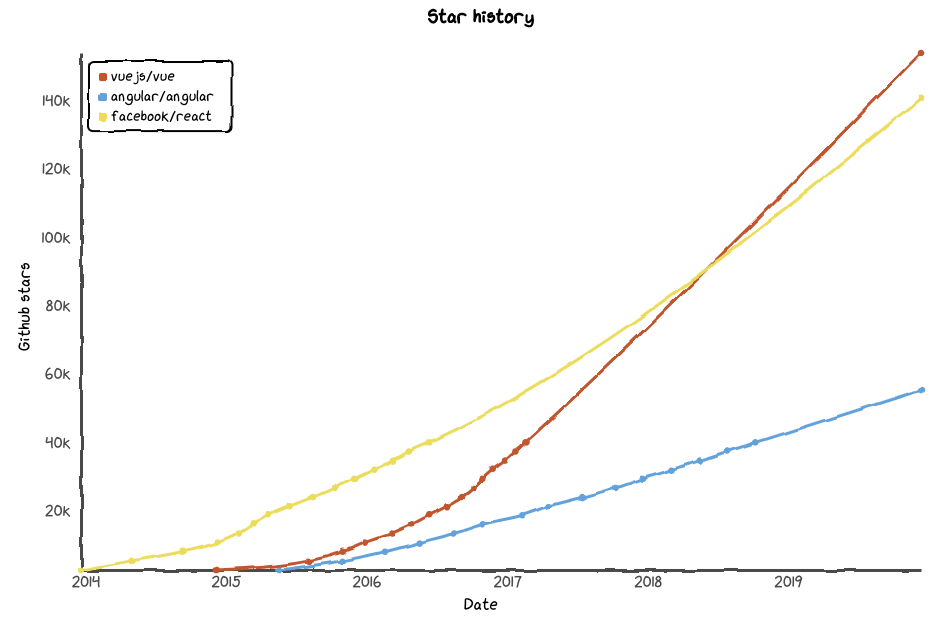
\includegraphics[scale=.4]{vuegithub.png}
            \caption{ Github stars ranking\cite{githubStars}}
    \end{center}
\end{figure}
\par 
A sudden shift in the number of stars of Vue occurred in mid-2016 and, recently, Vue has been up there with React among the most popular frameworks.
\begin{figure}[H]
    \begin{center}
        \label{abc}
            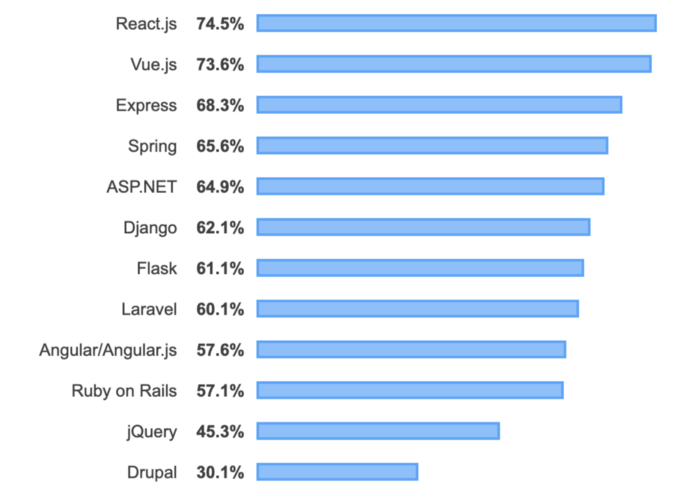
\includegraphics[scale=.4]{vue1.png}
            \caption{ Most loved framework\cite{vue-stackoverflow}}
    \end{center}
\end{figure}
\par React.js and Vue.js are both the most loved and most wanted web frameworks by developers. Major technology giants like google,apple and gitlab are started using Vue js for their front end development.
\begin{figure}[H]
    \begin{center}
        \label{abc}
            
\includegraphics[scale=.4]{vue2.png}
            \caption{ Major users of vue \cite{vue-users}}
    \end{center}
\end{figure}
\chapter{VUE IN DETAIL}

\section{FEATURES}



\paragraph{Virtual DOM:} 

Vue.js makes the use of virtual DOM, which is also used by other frameworks such as React, Ember, etc. The changes are not made to the DOM, instead a replica of the DOM is created which is present in the form of JavaScript data structures. Whenever any changes are to be made, they are made to the JavaScript data structures and the later it is compared with the original data structure. The final changes are then updated to the real DOM, which the user will see changing. This is good in terms of optimization, it is less expensive and the changes can be made at a faster rate.

\paragraph{Data Binding:}

The data binding feature helps manipulate or assign values to HTML attributes, change the style, assign classes with the help of binding directive called v-bind available with Vue.js.

\paragraph{Components:}

Components are one of the important features of Vue.js that helps create custom elements, which can be reused in HTML.

\paragraph{Event Handling:}

v-on is the attribute added to the DOM elements to listen to the events in Vue.js.

\paragraph{Animation/Transition:}

Vue.js provides various ways to apply transition to HTML elements when they are added/updated or removed from the DOM. Vue.js has a built-in transition component that needs to be wrapped around the element for transition effect.Third party animation libraries can also be added more interactivity to the interface.


\paragraph{Templates:}

Vue.js provides HTML-based templates that bind the DOM with the Vue instance data. Vue compiles the templates into virtual DOM Render functions. Template can be used to the render contents in web page

\paragraph{Directives:}

Vue.js has built-in directives such as v-if, v-else, v-show, v-on, v-bind, and v-model, which are used to perform various actions on the frontend.

\paragraph{Watchers:}

Watchers are applied to data that changes. For example, form input elements. Here, No need for any additional events. Watcher takes care of handling any data changes making the code simple and fast.

\paragraph{Routing:}

Navigation between pages is performed with the help of vue-router.

\paragraph{Lightweight:}

Vue.js script is very lightweight and the performance is also very fast

\paragraph{Vue-CLI:}

Vue.js can be installed at the command line using the vue-cli command line interface. It helps to build and compile the project easily using vue-cli.
\newpage
\section{Vue vs React}

\paragraph{Virtual DOM:}

Virtual DOM is a virtual representation of the DOM tree. With virtual DOM, a JavaScript object is created which is the same as the real DOM. Any time a change needs to be made to the DOM, a new JavaScript object is created and the changes are made. Later, both the JavaScript objects are compared and the final changes are updated in the real DOM.

Vue.js and React both use virtual DOM, which makes it faster.

\paragraph{Template v/s JSX:}

Vue.js uses html, js and css separately. It is very easy for a beginner to understand and adopt the Vue.js style. The template based approach for Vue is very easy.

React uses jsx approach. Everything is JavaScript for ReactJS. HTML and CSS are all part of JavaScript.

\paragraph{Installation Tools:}

React uses create react app and Vue uses vue-cli /CDN/npm. Both are very easy to use and the project is set up with all the basic requirements. React needs webpack for the build, where as Vue does not. Vue enables start with  coding anywhere in jsfiddle or codepen using the cdn library.

\paragraph{Popularity:}

React is popular than Vue. The job opportunity with React is more than Vue. There is a big name behind React i.e. Facebook which makes it more popular. Since, React uses the core concept of JavaScript, it uses the best practice of JavaScript. One who works with React will definitely be a very good with all the JavaScript concepts.

Vue.js is a developing framework. Presently, the job opportunities with Vue.js are less in comparison to React. According to a survey, many people are adapting to Vue.js, which can make it more popular in comparison to React and Angular. There is a good community working on the different features of Vue.js. The vue-router is maintained by this community with regular updates.

Vue.js has taken the good parts from Angular and React and has built a powerful library. Vue.js is much faster in comparison to React/Angular because of its lightweight library.

\chapter{VUE.JS INSTALLATION }
There are many ways to install Vue.js. The easy method is by using Vue.js file from the CDN library. Vue can also be  installed  from npm (node pacakge magager). The command line interafce of Vue is also available in npm.
\section{VUE.JS INSTALLATION USING CDN}
The easiest and quickest way of installing Vue is by directly including Vue via a CDN (Content Delivery Network) in a script tag. This means that instead of Vue residing on your own server, it will be delivered from a separate server.
\begin{figure}[H]
    \begin{center}
        \label{abc}
            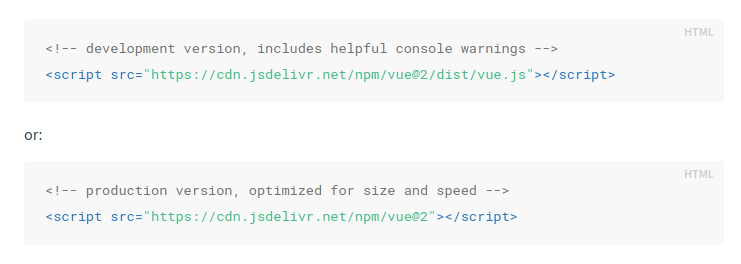
\includegraphics[scale=.6]{vueSetup.png}
            \caption{ Vue.js setup using CDN \cite{vue-code}}
    \end{center}
\end{figure}

\section{VUE.JS INSTALLATION USING NPM}
For large scale applications with VueJS, it is recommended to install using the npm package. It comes with Browserify and Webpack along with other necessary tools, which help with the development. Following is the command to install using npm.
\begin{lstlisting}
npm install vue

\end{lstlisting}
\chapter{VUE DIRECTIVES}
A directive is some special token in the markup that tells the library to do something to a DOM element. Vue.js has built-in directives such as v-if, v-else, v-show, v-on, v-bind, and v-model, which are used to
perform various actions on the frontend
\paragraph{v-if}
The directive v-if is used to conditionally render a block.
The block will only be rendered if the directive’s expression returns a truthy value.
\paragraph{v-for}

The directive v-for to render a list of items based on an array
\paragraph{v-on}

 v-on directive can be used  to listen to DOM events and run some JavaScript when they’re triggered.

\paragraph{v-model}

The v-model directive is used to create two-way data bindings on form input, textarea, and select
elements.
It automatically picks the correct way to update the element based on the input type.
\paragraph{v-show}
Another option for conditionally displaying an element is the v-show directive. The usage is largely the same v-if
\chapter{VUE SYNTAX }
\section{Hello World}
\begin{figure}[H]
    \begin{center}
        \label{abc}
            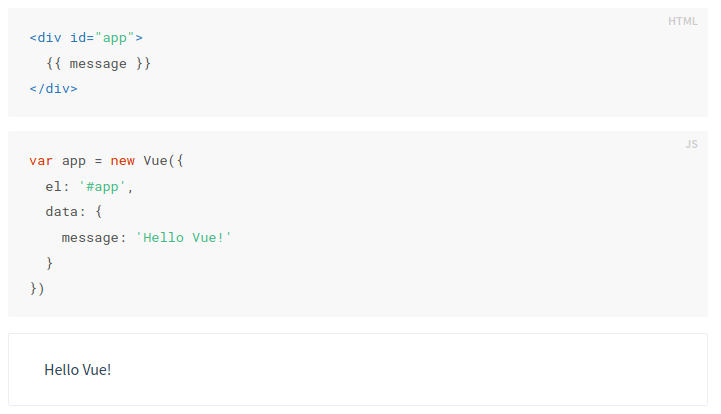
\includegraphics[scale=.6]{vueHelloWorld.png}
            \caption{Hello World in Vue.js \cite{vue-code} }
    \end{center}
\end{figure}
There is a div which is added in the body that prints “Hello Vue” in the browser. A message is also added in an interpolation, i.e. \{\{\}\}. This interacts with Vue.js and prints the data in the browser. To get the value of the message in the DOM, An instance of vuejs must be created.
\section{CONDITIONAL RENDERING}
\begin{figure}[H]
    \begin{center}
        \label{abc}
            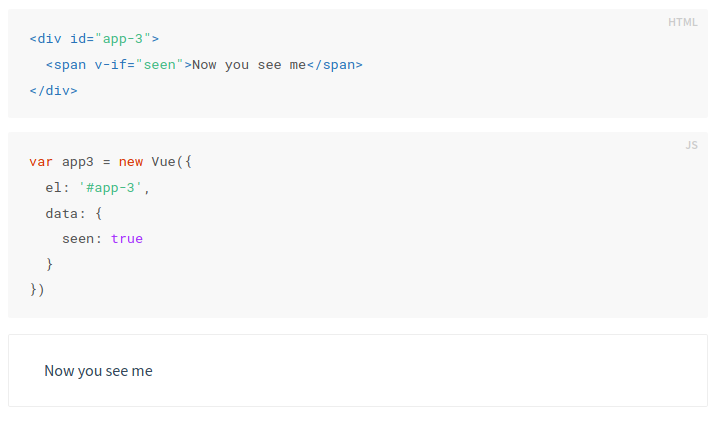
\includegraphics[scale=.6]{v-if.png}
            \caption{Conditional rendering in Vue.js \cite{vue-code}  }
    \end{center}
\end{figure}
Span element will only be rendered if value of "seen" is set to True. Otherwise the message "Now you see me" will disappear.
\section{Using Loop in Vue}
\begin{figure}[H]
    \begin{center}
        \label{abc}
            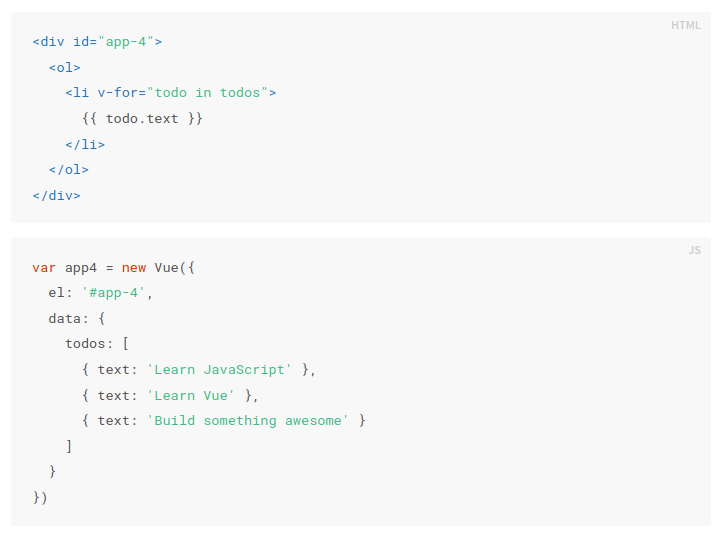
\includegraphics[scale=.6]{v-for.png}
            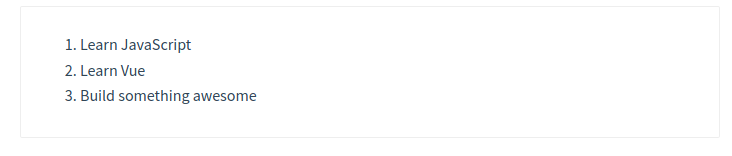
\includegraphics[scale=.6]{v-forOutput.png}
            \caption{Using v-for directive  in Vue.js \cite{vue-code} }
    \end{center}
\end{figure}
\begin{center}
    
\end{center}
    v-for directive can be used for displaying a list of items using the data from an Array:
    
\section{Handling user input in Vue}  
\begin{figure}[H]
    \begin{center}
        \label{abc}
            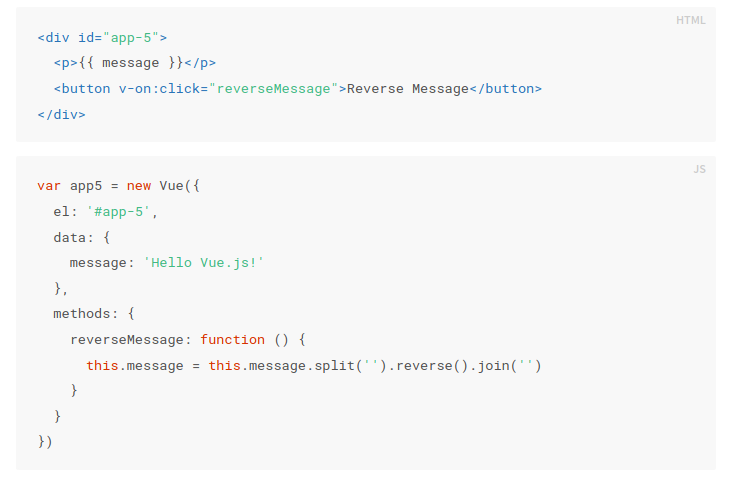
\includegraphics[scale=.6]{v-on.png}
            
\includegraphics[scale=.6]{v-onOutput.png}
            \caption{Using v-on directive  in Vue.js \cite{vue-code} }
    \end{center}
\end{figure}
\begin{center}
    
\end{center}
v-on directive is used  to attach event listeners that invoke methods on our Vue instances. When a user clicks on the button the message "Hello Vue!" will get reversed
\newpage 
\section{Vue component}
The component system is another important concept in Vue, because it’s an abstraction that allows us to build large-scale applications composed of small, self-contained, and often reusable components. Almost any type of application interface can be abstracted into a tree of components.
\begin{center}
    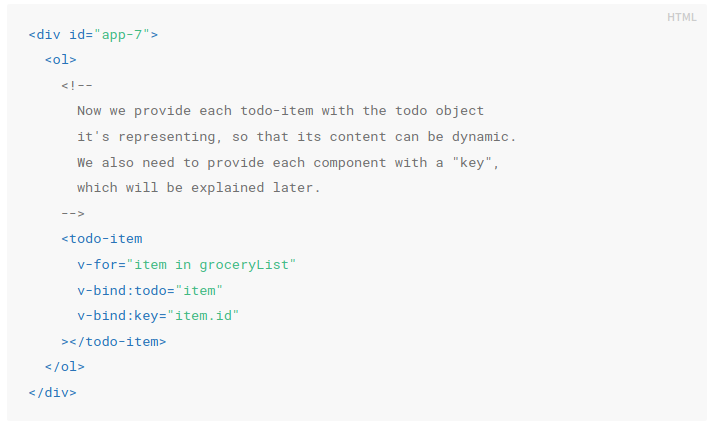
\includegraphics[scale=.6]{v-comp.png}
\end{center}
In the js part a component named todo-item can declared and it can be rendered as many times the developer wants with help of an array. This concept helps to reuse the code and improve performance. 
\begin{figure}[H]
    \begin{center}
        \label{abc}
            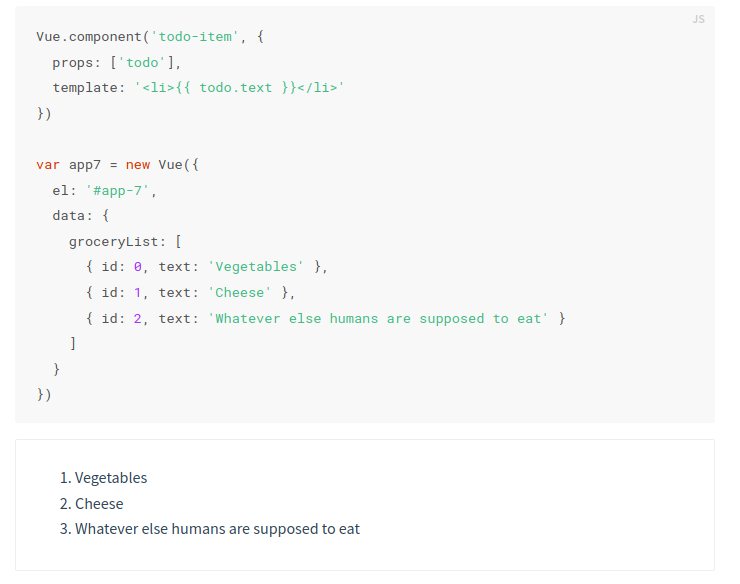
\includegraphics[scale=.6]{v-comp1.png}
            \caption{Using Vue component\cite{vue-code} }
    \end{center}
\end{figure}
\chapter{ADVANTAGES AND DISADVANTAGES}
\section{Advantages}
\paragraph{Very Small Size:}
The success of JavaScript framework depends on its size. The
smaller the size is, the more it will be used. One of the greatest
advantages of Vue.js is its small size. The size of this framework
is 18–33KB and it takes no time for the user to download and use
it. This does not mean that it has low speed because of small size.
Instead, it beats all the bulky frameworks like React.js, Angular.js,
and Ember.js.
\paragraph{Easy to Understand and Develop Applications:}
One of the reasons for the popularity of this framework is that it is
quite easy to understand. The user can easily add Vue.js to his web
project because of its simple structure. Both the small as well as
large scales templates can be developed through this framework
which saves a lot of time. In case of any problem, the user can
easily trace the blocks with errors. All this is because of its simple
structure.
\paragraph{Simple Integration:} Vue.js is also popular among the web developers because it
facilitates them to integrate with the existing applications. This is
because it is based on JavaScript framework and can be integrated
into other applications built on JavaScript. This means that it is
useful for developing new web applications as well as altering the
pre-existing applications. This integration is possible because
Vue.js has components for everything.
\paragraph{Detailed Documentation:}
Developers always like to use the framework with detailed
documentation because it is always easy for them to write their
first application. The documentation with Vue.js is so
comprehensive that any user who knows a little about JavaScript
and HTML can develop his own application or web page.
\paragraph{Flexibility:}
A great deal of flexibility is another advantage of Vue.js. It allows
the user to write his template in HTML file, JavaScript file, and
pure JavaScript file using virtual nodes. This flexibility also makes
it easy to understand for the developers of React.js, Angular.js,
and any other new JavaScript framework. Vue.js has proved a lot
beneficial in the development of those simple applications that run
directly from browsers.
\section{Disadvantages}
\paragraph{Less Plugins/Components:}

Common plugins are useful as they work with various other tools to make development easy. Vue.js does not have most of the common plugins, and that is the drawbacks of Vue.js.

\paragraph{Vue.js Evolving Fast:}

What is working in Vue today may be outdated tomorrow. This is the most significant drawbacks of Vue as developers find it is rather complicated, and they have to learn the framework quite frequently.


\paragraph{Small Community:}

Vue was initially launched in 2014, and therefore it is still new and evolving very fast. But community is small compared to react.
\chapter{CONCLUSION}

\begin{itemize}

\item Vue is a progressive framework for building user interfaces. 
\item The core library is focused on the view layer only, and is easy to pick up and integrate with other libraries or existing projects.  
\item Vue is also perfectly capable of powering complex Single-Page  Applications.
\item Vue is more simple and flexible.
\item Vue allows to make just a specific part of the application
\item The vue community is small compared to react.
\item Vue.js does not have most of the common plugins, and that is the drawbacks of Vue.js.


\end{itemize}

%\chapter{REFERENCES}
\renewcommand{\bibname}{\uppercase{REFERENCES}}
\begin{thebibliography}{999}
\addcontentsline{toc}{chapter}{\hspace{0.19in} REFERENCES}



\bibitem{vue-code}{https://vuejs.org/v2/guide/index.html 
 }
\bibitem{a}{https://www.tutorialspoint.com/vuejs/index.htm 
  }
\bibitem{a}{https://en.wikipedia.org/wiki/Vue.js
  }
\bibitem{a}{https://medium.com/@ronak8036/pros-and-cons-of-the-vue-js-framework-8015dcbc05ef
  }
  \bibitem{githubStars}{https://gist.github.com/tkrotoff/b1caa4c3a185629299ec234d2314e190
  }
  \bibitem{a}{https://towardsdatascience.com/what-are-the-pros-and-cons-of-using-vue-js-3689d00d87b0s
 }
  \bibitem{vueLogo}{https://www.baymediasoft.com/blog/developers/vue-js-framework-is-making-development-easier} 
  
  \bibitem{vue-stackoverflow}{https://medium.com/hackernoon/angular-vs-react-vs-vue-which-is-the-best-choice-for-2019-16ce0deb3847}
  
  \bibitem{vue-users}{https://medium.com/notonlycss/google-apple-and-other-users-of-vue-js-e4505359e5d5}
 












\end{thebibliography}

\end{document}